\documentclass[12pt, a4paper]{article}
\usepackage{latexsym, listings, graphicx, hyperref}


\lstset{language=bash}  

\newtheorem{theorem}{Theorem}
\newtheorem{definition}{Definition}

\renewcommand{\baselinestretch}{1.3} % 1.5 denotes double spacing. Changing it will change the spacing

\setlength{\parindent}{0in} 

\begin{document}
\title{Testing Raspberry Pi  based \\ microscope camera \\ on  growth
  of \\  household yeast}
\author{Bjørn Remseth}
\date{28. mar. 2016}
\maketitle
\abstract{This document describes an experiment where yeast cells are
  grown on a microscope slide to test the microscope image capture
  mechanism, and inspire the author to get some ideas about how to
  capture even more interesting pictures of yeast growing.}

\section{Introduction}

Some time ago I installed microscope adapter on my Amscope
microscope.   Since then I have not tested if it is indeed useful to
capture time series of microscrope, so today I decided I should test
that. 

As an experimental system, I started up an image capture programme in
the Pi, and prepared a solution of yeast and sugar on a microscope
slide, and set about to capture images what happened.

This note describes the experimental system, the experimental
protocol, and makes some suggestions on how to improve the
experimental protocol for future experiments.

\section{Methods and materials}

\begin{figure}[th]
\begin{center}
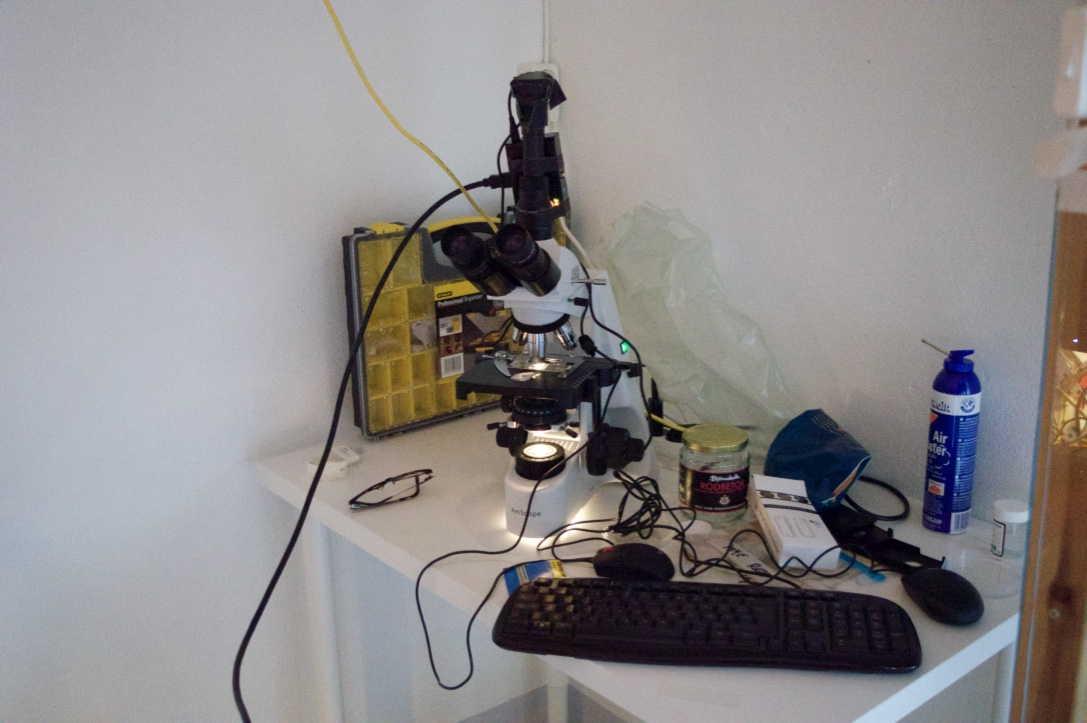
\includegraphics[width=10cm]{images/experimental_setup.jpg}
\caption{The experimental setup captured during the experiment.}
\label{lastimage}
\end{center}
\end{figure}


A yeast/sugar/water solution was made by adding about a teaspoon of
sugar to an egg-glass of water and stirring.  The solution was then
cooled by adding tapwater.  To this solution a small amount (roughly
equivalent to 30 \(mm^3\) of household yeast (``IDUN mors hjemmebakte
original gjær'' with a ``best before'' marking of april 10 2016).

A drop of this solution was put onto a microscope slide (``Elka
Assistent, Objektträger micro slides  cleaned'') and then put onto the
microscope and a cover glass was put on top.   The solution spread out
under the entire cover glass and on visual inspection it seemed to be
completely uniform.

The slide was then put onto the microscrope.  The microscope is an
Amscope 40X-2500X Infinity  trinocular compound microscope.   The 40x
microscope lens (air, not oil) was selected.   

To this microscope was connected a 5 megapixel raspberry Pi camera
module connected to a Raspberry Pi 2 model B.   The camera sensor was
connected to the microscope using a 3D printed adapter. The Raspberry
Pi module was then connected  to the microscope iself using duct tape
(also know as ``gaffa tape'').  The 3D printed sensor/microscope adapter was
printed using red plastic, so to avoid light leaking in to the sensor
thorugh the plastic, the entire adapter was covered in black duct tape.

The Raspberry pi is a linux based computer.  To focus it on the slide,
I used the ``raspstill -t 0'' program to show a large live capture
image on the attached HDMI screen.   When focus was determined to be
adequate, a script was used to capture frames:

\begin{lstlisting}[frame=single]
mkdir -p /home/pi/yeast

while /bin/true ; do 
    DATE=$(date +"%Y-%m-%d_%H%M%S")
    raspistill -vf -hf -o /home/pi/yeast/images/$DATE.jpg
    echo "Captured picture at $DATE"
    sleep 30
done
\end{lstlisting}

This script was run using the "nohup" utility to ensure that it
continued running even if the network connection to the Raspberry Pi
was lost during the experiment.

The frames were then converted to an mp4 movie.   

To refer to the captured frames I used the following script to create
symbolic links that pointed to the original frames, but were numbered
in a manner recognisable by the avconv program

\begin{lstlisting}[frame=single]
FOO=1; 
for x in images/* ; do 
    ln -s ../$x $(printf "frames/%06d.jpg" $FOO) ;
    FOO=$(expr $FOO + 1) ; 
done
\end{lstlisting}

First attempted to to perform the conversion on the Raspberry Pi using
the command:

\begin{lstlisting}[frame=single]
avconv -r 10 -i  frames/%06d.jpg   \
     -r 10 -vcodec libx264 -crf 20    \
     -g 15   timelapse.mp4 
\end{lstlisting}


This did not succeed due to a lack of available memory.  Instead I
then transfered the files to a computer running OSX using the ``scp''
command 

\begin{lstlisting}
scp 'pi@10.0.0.23:/home/pi/yeast/images/*' . 
\end{lstlisting}

and then ran the ``ffmpeg'' encoder to produce an mp4 movie file:

\begin{lstlisting}
ffmpeg -i frames/%06d.jpg timeseries.mp4 
\end{lstlisting}

During the work with the development of the symbolic link generating
script, I made the mistake of deleting all of the images (instead of
``frames''), so about an hour of captured images were lost.


\section{Results}

\begin{figure}[th]
\begin{center}
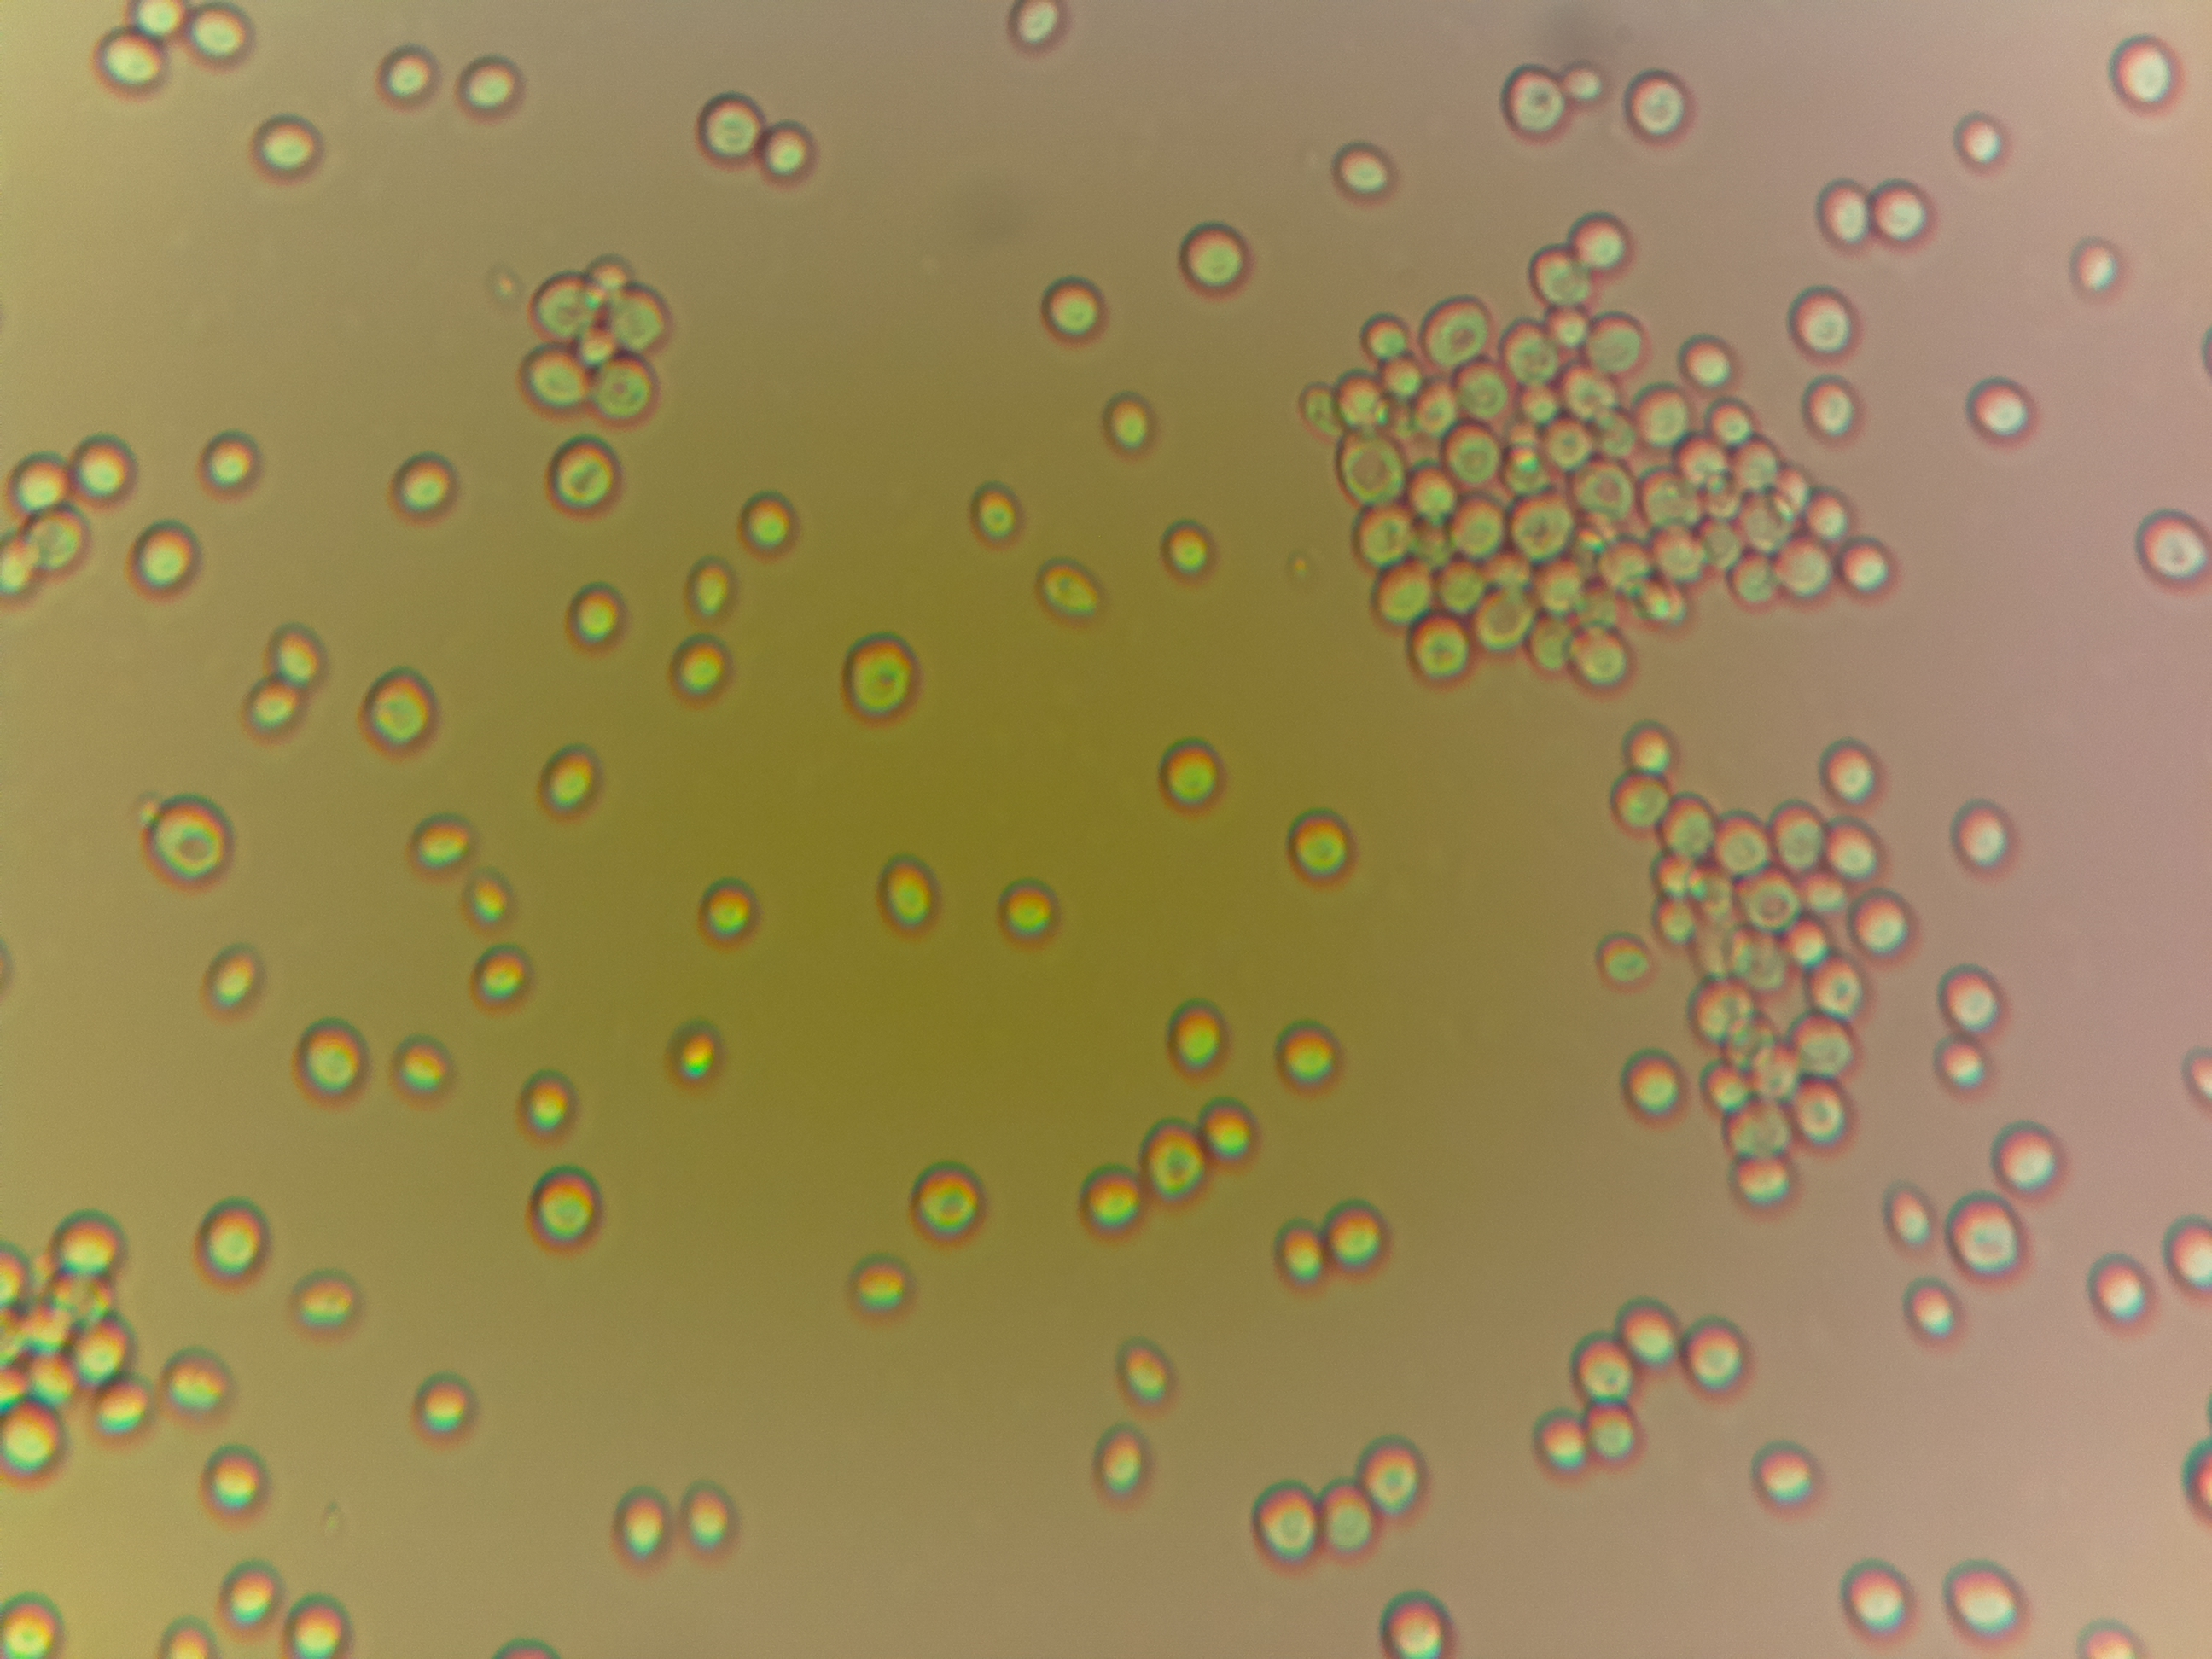
\includegraphics[width=10cm]{images/2016-03-28_111108.jpg}
\label{firstimage}
\caption{The first image in the sequence 2016-03-28\_111108.jpg}
\end{center}
\end{figure}


\begin{figure}[th]
\begin{center}
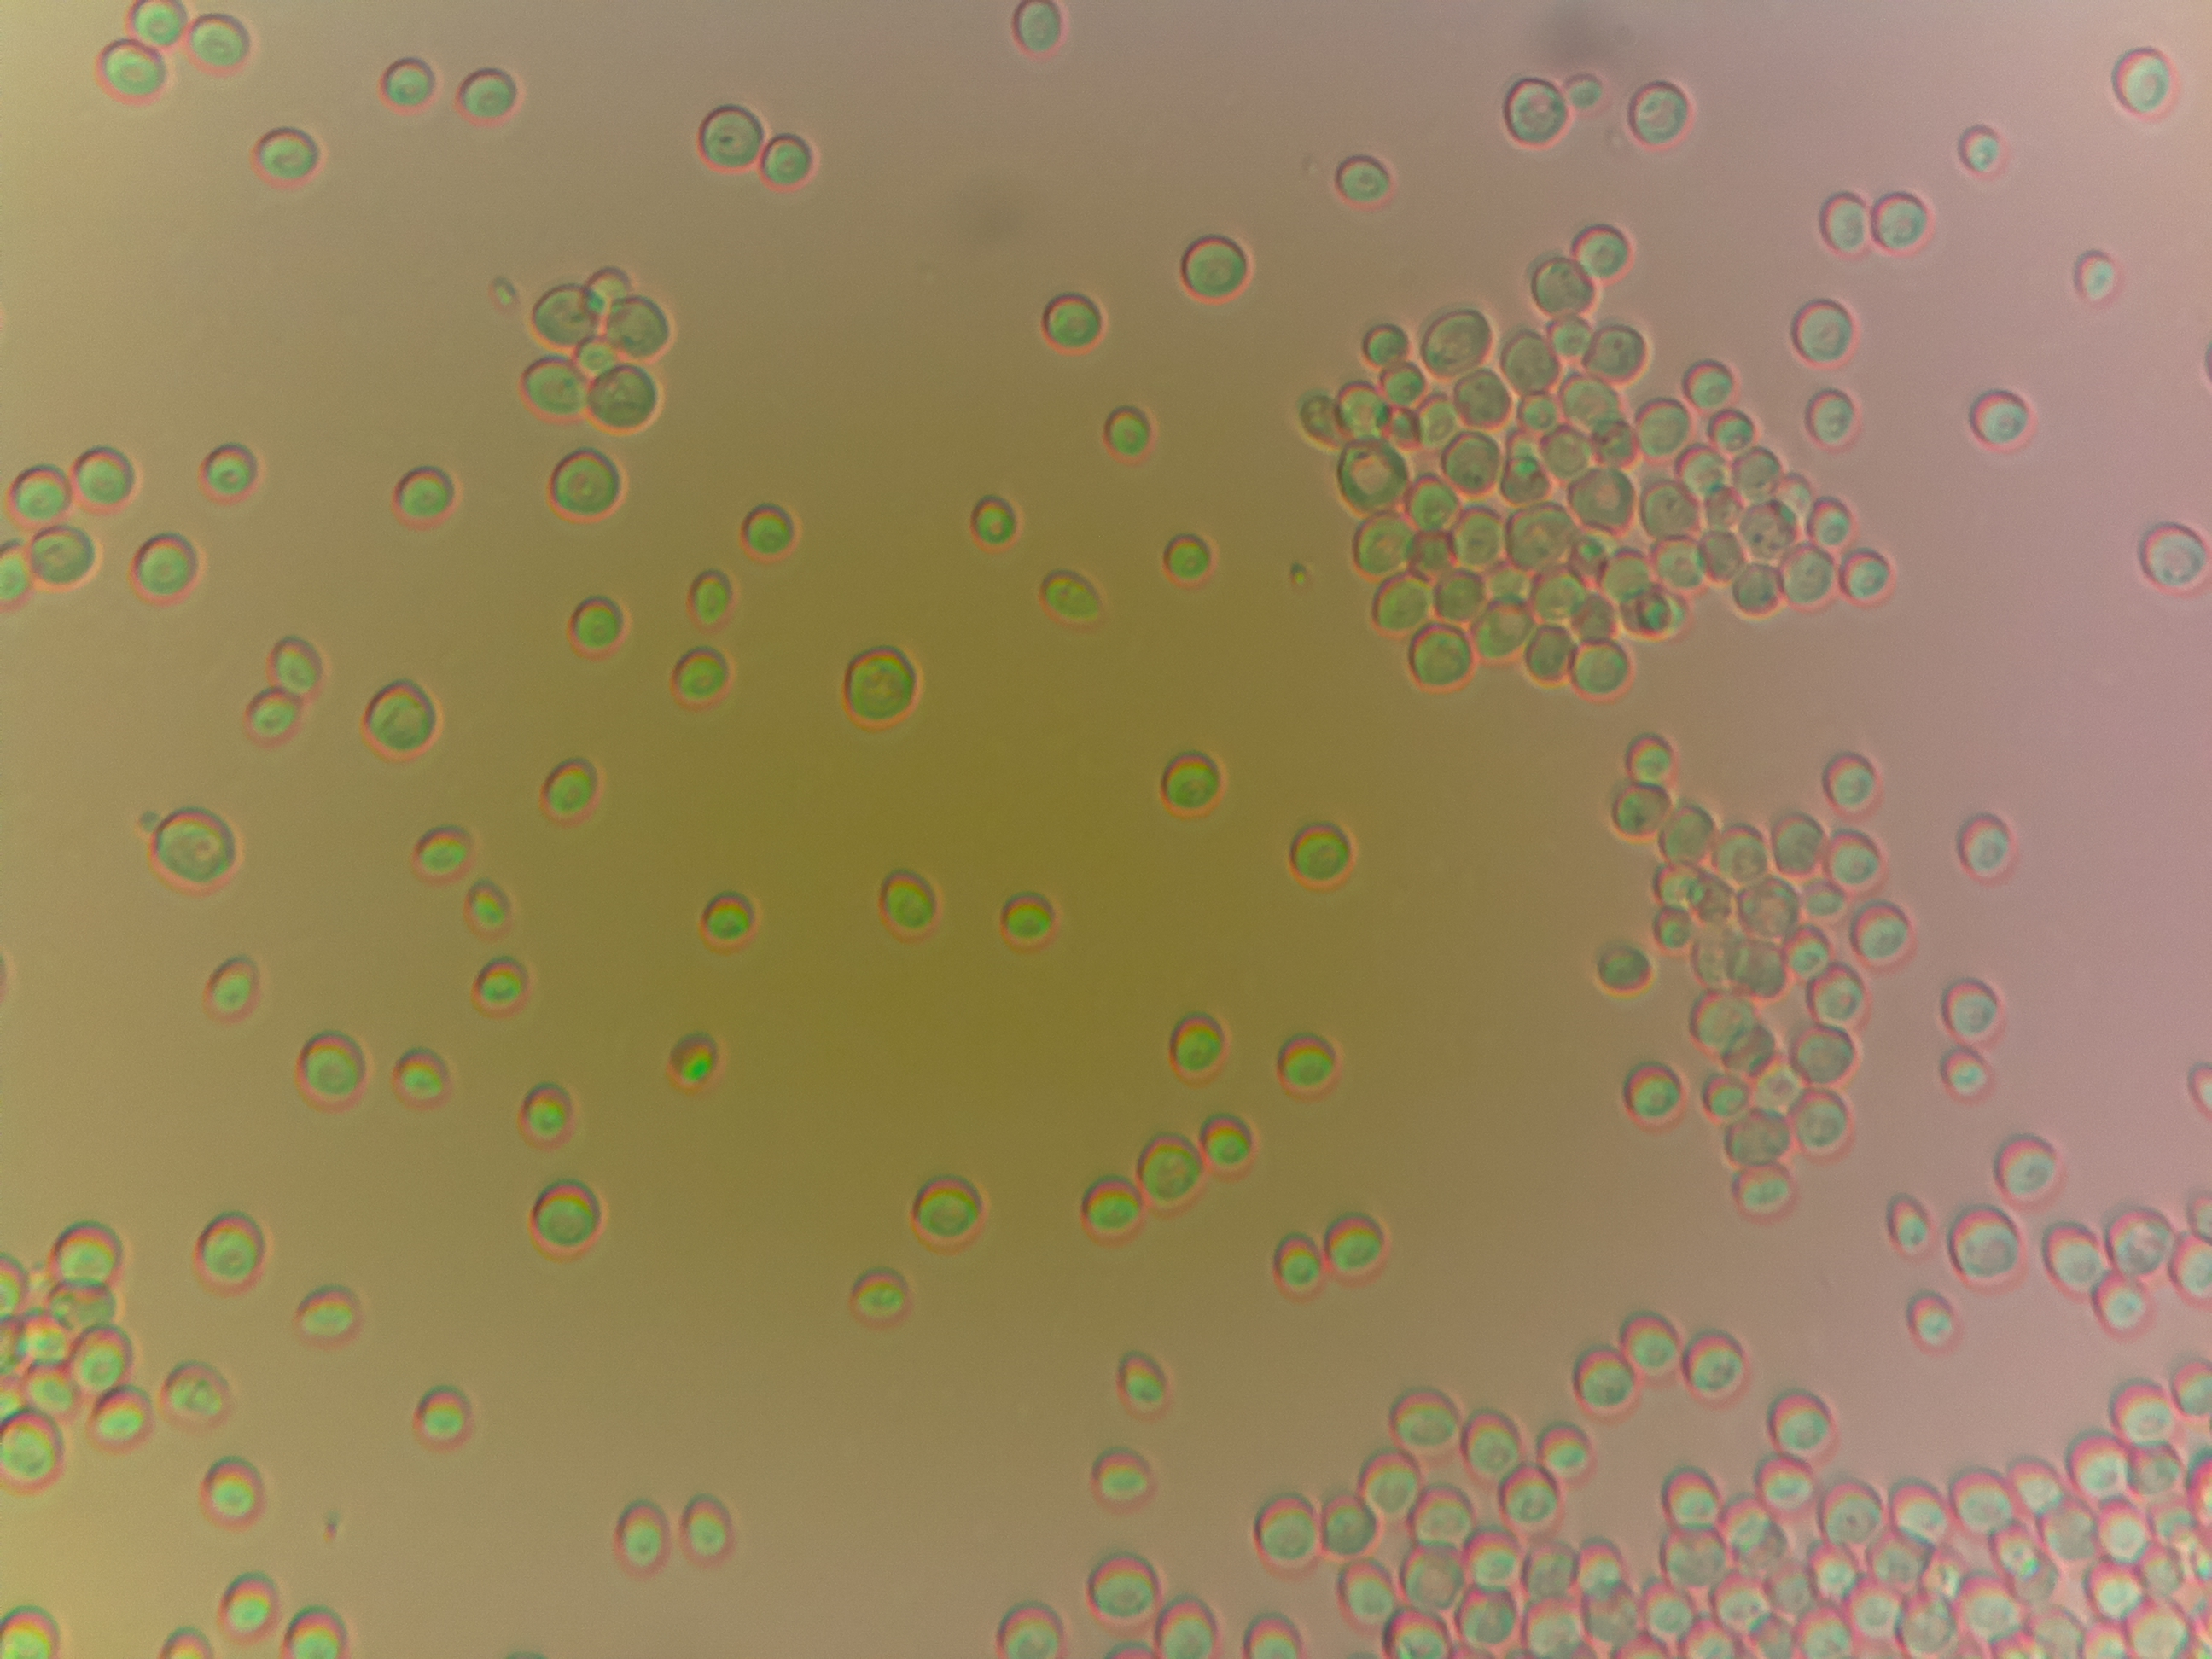
\includegraphics[width=10cm]{images/2016-03-28_140625.jpg}
\label{lastimage}
\caption{The last image in the sequence 2016-03-28\_140625.jpg}
\end{center}
\end{figure}

During the experiment, and excluding the hour or so of frames that
were lost, 336 frames were captured.  The first and last images can be
found in figures \ref{firstimage} and \ref{lastimage}. 

All of the frames and the movie produced using ffmpeg were then placed
in a pair of dropbox\footnote{The yeast growth movie: 
\url{https://dl.dropboxusercontent.com/u/187726/shared-experimental-data/yeast-growth-28-mar-2016/movies/yeast-growth.mp4}.}
\footnote{The raw image data: 
\url{https://www.dropbox.com/sh/89nr05c739ucmcs/AADHEj9F1bnCn4t480C_s9tsa?dl=0}.}.


\section{Discussion}

So that was fun :-)   It shows that there is some potential here.
Notes:  The movie shows

When watching the movie I could not see cell division occuring, but I
did see movement inside the cells, and that \emph{could} be mitosis and
cromosomes being pulled to the spindles of the cells, but that should
be confirmed and studied a bit more before I quite believe it.

I can observe that cells grow to about twice their original size
during the movie.

At the end of the sequence there is an onrush of cells from the
bottom.  One explanation could be that there has been more successful
cell division elsewhere on the slide, and that cells resulting from that division
is being pushed into the part viewed during the experiment.

There is a bunch of things we can do that could be intersting in the
future. Here are the ones I remember while writing this document.

\begin{itemize}
\item The yellow color is a bit annoying.  Perhaps fixing the color
  balance either post-capture or by putting a filter into the
  light source would improve the images?
\item The time spent during this experiment was not enough to 
  se an actual cell division, so just running the experiment for 
  a longer time (more than three hours) is probably something that
 should be tried.
\item Growth is influenced by both nutrient (sugar) availability and
  temperature.   Using another nutrient (fructose or glucose) could
  be interesting.  It could also be interesting to increase the
  temperature, or at the very least measure the temperature of the
  experimental assembly during the experiment.
\item A test run focusing only on a few cells but with higher
  magnification (e.g. 100 oil) could possible give more details on the cell division
  cycle, perhaps allowing confirmation / rejection of the hypothesis
  that we actually saw chromosomes being pulled apart.
\item Using the raw images there are multiple kinds of analysis that
  can be attampted:
\begin{itemize}
 \item Identify cells, their locations and size.
 \item Track movement, division and perhaps interior content
   (e.g. visible chromosomes) over time.
 \item Using e.g. ijulia or ipython would be fun.
\end{itemize}
\item Adding date/time to the images would be useful both for later
  analysis and to avoid confusion in general :-)
\item Being more precise when preparing the yeast/nutrient solution
  would also be useful, so that it was repeatable and therefore
  tunable for better yield (or whatever I want to test).
\end{itemize}




\section{References}


Watching bread yeast make bubbles: 
http://www2.mrc-lmb.cam.ac.uk/microscopes4schools/yeast.php


\end{document}